\documentclass{../res/univ-projet}

%Import des packages utilisés pour le document
\usepackage[utf8x]{inputenc}
\usepackage[francais]{babel}
\usepackage[T1]{fontenc}
\usepackage{lscape}
%\usepackage{array}
%\usepackage{hyperref}
%\usepackage{tabularx, longtable}
%\usepackage[table]{xcolor}
%\usepackage{fancyhdr}
%\usepackage{lastpage}


\definecolor{gris}{rgb}{0.95, 0.95, 0.95}

%Redéfinition des marges
%\addtolength{\hoffset}{-2cm}
%\addtolength{\textwidth}{4cm}
\addtolength{\topmargin}{-1cm}
\addtolength{\textheight}{1cm}
\addtolength{\headsep}{0.8cm} 
\addtolength{\footskip}{-0.2cm}

%Import page de garde et structures pour la gestion de projet
%\usepackage{structures}
%Variables
\logo{../res/logo_univ.png}
\title{Spécification Technique de Besoin}
\author{Kheireddine \bsc{Berkane}, Nasser \bsc{Adjibi}}
\projet{Compilateur LLVM}
\projdesc{Langage jouet Kawa}
\filiere{M1GIL - Conduite de Projet}
\version{0.7}
\relecteur{Pierre-Luc \bsc{BLOT}, Alexandre \bsc{PETRE}}
%\signataire{Florent \bsc{NICART}}
\date{\today}

\histentry{0.1}{04/11/2014}{Version initiale.}
\histentry{0.1.5}{18/11/2014}{Définition des cas d'utilisations et des exigences.}
\histentry{0.2}{03/12/2014}{Modifications par rapport au retour client du 25/11/2014.}
\histentry{0.3}{10/12/2014}{ \begin{itemize}
								 \item Les parties événements déclenchants ont été détaillées.
								 \item Les parties flots d'exceptions, ainsi que les conditions d’arrêts de toutes les exigences fonctionnelles ont été détaillées.
								 \item L'ajout des exigences opérationnelles d'interface.
								 \item Correction des erreurs signalées lors de la réunion client 04/12/2014.	
							 \end{itemize}	 	
								 }
\histentry{0.4}{22/12/2014}{ \begin{itemize}
\item Les parties événements déclenchants ont été modifiées et structurées sous forme d'une liste.
\item Les parties flots d'exceptions, ainsi que les conditions d’arrêts de toutes les exigences fonctionnelles ont été été modifiées et structurées sous forme d'une liste.
\item La suppression des exigences opérationnelles d'interface après une remarque faite par le prof du TP gestion de projet.
\item Changement de priorité de l'exigence fonctionnelle EF\_4 en secondaire car elle dépend de l'exigence EF\_3 qui est secondaire.
\item Correction des erreurs signalées lors du retour client par mail le 19/12/2014.	
\end{itemize}	 	
}
\histentry{0.5}{18/01/2015}{ \begin{itemize}
\item Élimination des exigences de réalisations qui correspondent aux exigences fonctionnelles afin d'éviter les redondances inutiles. 
\item La partie des exigences fonctionnelles a été détaillée ainsi que les scénarios des exceptions ont été spécifiés afin de faciliter les tests après.
\item Modifications apportées par rapport à la revue du lancement du projet 19/01/2015.
\end{itemize}
}
\histentry{0.6}{11/04/2015}{ 
\begin{itemize}
\item Élimination de l'exigence fonctionnelle EF\_3 : Compiler une application en mode partagé 
\item Élimination de l'exigence fonctionnelle EF\_4 : Compiler une bibliothèques partagée
\item Élimination de l'exigence fonctionnelle EF\_6 : Indiquer les chemins des dépendances entre le source de l'application et des modules (classe/interface) externes
\item Élimination de l'exigence de réalisation EXR\_4 : Compilation d'application partagée
\item Élimination de l'exigence de réalisation EXR\_6 : Compilation de bibliothèque partagée
\item Élimination de l'exigence de réalisation EXR\_25 : Définition d'attributs ou de variables de type \textbf{value}
\item Élimination de l'exigence de réalisation EXR\_26 : Définition méthode value
\item Élimination de l'exigence de réalisation EXR\_41 :  Gestion des exceptions
\item Changement du diagramme de cas d'utilisation après la discussion avec client afin de réduire quelques exigences fonctionnelles et de réalisation 
\end{itemize}
}

\newpage
\histentry{0.7}{15/04/2015}{ 
\begin{itemize}
\item Mettre l'exigence fonctionnelle EF\_3 : Afficher la version du compilateur en secondaire
\item Élimination de l'exigence fonctionnelle EF\_4 :Activer l'affichage en couleur
\item Élimination de l'exigence de réalisation EXR\_5 : Garbage collector
\end{itemize}
}


% -- Début du document -- %
\begin{document}

%Page de garde
\maketitle
\newpage
%La table des matières
\tableofcontents
\newpage

\section{Contexte du projet}
  \subsection{Origine du projet}
    L'objectif à travers le choix du langage \textbf {kawa} qui est similaire à
    \textbf {java} (un langage de haut niveau d'abstraction) c'est de permettre
    une facilité ainsi qu'une rapidité de développement par rapport à d'autres 
    langages de programmation tel que le «C». Le code Java  est compilé dans un langage intermédiaire  Bytecode et est exécuté dans un environnement 
    d'exécution JVM (Java Virtual Machine), dans le cadre de notre projet nous 
    allons montrer que l'on peut compiler un code similaire à java (kawa) en 
    code natif sans passer par une machine virtuelle (MV).

  \subsection{Contexte de développement}
    Ce projet s'sincrit dans le cadre de la formation Master 1 Génie de l'Informatique Logicielle dispensée à l'UFR des Sciences et Techniques de Saint Etienne du Rouvray. Il nous a été proposé par nos professeurs référents, notamment Mr Nicart. Pour cela, nous disposons d'environ 11 semaines pour réaliser tous les documents techniques, et d'un peu plus de 15 semaines pour le développement.\\

      Ce projet nous été proposé le 17/10/2014. Notre équipe de développement est composée de sept membres:
      \begin{itemize}
        \item ADJIBI Nasser 
        \item PETRE Alexandre
        \item TASSERIE Majid
        \item BLOT Pierre-Luc
        \item BERKANE Kheireddine
        \item IDRISSOU Hamzath
        \item AHOUATE Abdellatif
      \end{itemize}
      \vspace{5mm}
      Le 16/02/2015 un membre à quitté l'équipe. Elle est désormais composée des membres suivant:
      \begin{itemize}
        \item ADJIBI Nasser 
        \item PETRE Alexandre
        \item BLOT Pierre-Luc
        \item BERKANE Kheireddine
        \item IDRISSOU Hamzath
        \item AHOUATE Abdellatif
      \end{itemize}
      \vspace{5mm}
      \hspace{5mm}
      \begin{tabular}{
        |>{\centering}p{7,5cm}
        |>{\centering}p{7,5cm}|}
          \hline
          \color{white}\cellcolor{blue}\bfseries{Dates}&
          \color{white}\cellcolor{blue}\bfseries{Sujets}\\
          \cr
          \hline
          17/10/14     &   Remise du sujet    
          \cr
          \hline
          23/10/14     &   Première réunion client    
          \cr
          \hline
          03/11/14     &   Deuxième réunion client 
          \cr
          \hline
          14/11/14     &   Troisième réunion client 
          \cr
          \hline
          20/11/14     &   Quatrième réunion client 
          \cr
          \hline
          26/11/14     &   Cinquième réunion client 
          \cr
          \hline
          05/12/14     &   Sixième réunion client 
          \cr
          \hline
          22/12/14     &   Dernière réunion client 
          \cr
          \hline
          03/01/15     &   Remise des documents
          \cr
          \hline
          19/01/15     &   Revue de lancement du projet
          \cr
          \hline
    \end{tabular}\\

    Et les dates clés du projet pendant la phase de développement:

    \begin{tabular}{
        |>{\centering}p{7,5cm}
        |>{\centering}p{7,5cm}|}
          \hline
          \color{white}\cellcolor{blue}\bfseries{Dates}&
          \color{white}\cellcolor{blue}\bfseries{Sujets}\\
          \cr
          \hline
          19/04/15     &   Premier livrable
          \cr
          \hline
          24/04/15     &   Second livrable
          \cr
          \hline
          % todo : il manque la date de la présentation orale
    \end{tabular}\\

  \subsection{Les principaux acteurs}    
    \begin{tabular}{
        |>{\centering}p{7,5cm}
        |>{\centering}p{7,5cm}|}
          \hline
          \color{white}\cellcolor{blue}\bfseries{Rôles}&
          \color{white}\cellcolor{blue}\bfseries{Acteurs}\\
          \cr
          \hline
          Client  & Mr Nicart
          \cr
          \hline
          Professeur référent & Mr Nicart
          \cr
          \hline
          Equipe de développement & ADJIBI Nasser; PETRE Alexandre; BLOT Pierre-Luc; BERKANE Kheireddine; IDRISSOU SOULER Hamzath; AHOUATE Abdellatif
          \cr
          \hline
    \end{tabular}\\
  \subsection{Objectifs pousuivis}
    L'objectif du projet kawa est de livrer un compilateur fonctionnant avec la technologie LLVM au client au mois de Mai 2015. Ce projet va permettre à l'ensemble de notre groupe de travailler ensemble durant ces semaines et de développer ainsi nos compétences dans les technologies C++ et LLVM ainsi que ELF pour UNIX.
  \subsection{Documents de référence}
    \begin{tabular}{
        |>{\centering}p{7,5cm}
        |>{\centering}p{7,5cm}|}
          \hline
          \color{white}\cellcolor{blue}\bfseries{Nom du document}&
          \color{white}\cellcolor{blue}\bfseries{Description}\\
          \cr
          \hline
          STB.pdf & Ce document regroupe les attentes du client et établit une référence.
          \cr
          \hline
          ADR.pdf & Ce document rescence les difficultés qui pourraient ralentir la bonne avancée du projet.
          \cr
          \hline
          DAL.pdf & Ce document traduit les solutoins techniques conçue pour répondre aux exigences définies dans le document STB.pdf.
          \cr
          \hline
          CDR.pdf & Ce document définit les moyens et précédés mis en oeuvre pour assurer la recette du logiciel développé.
          \cr
          \hline
    \end{tabular}\\
%% ------ Fin section ---------------------------------------------------------

\section{Méthodologie de développement}
  \subsection{Méthode de développement}
    Le projet va être développé en s’appuyant sur les méthodes agiles. Nous avons décidé de nous appuyer notamment sur deux de ces méthodes : la méthode DSDM (Dynamic Systems Development Method) ainsi que la méthode XP (eXtrem Programming). En effet, nous allons produire différentes versions du logiciel. Lors de chaque version, de nouvelles fonctionnalités seront ajouter afin d’arriver à la version finale comprenant toutes les fonctionnalités demandées par le client. Voici les points sur lesquels vont reposer notre projet :
    \begin{itemize}
      \item La communication : Ce projet est un travail d’équipe.
      \item La simplicité : Une solution doit uniquement répondre au problème posé.
      \item Le feedback : L’avancement sera évalué sur des éléments concrets régulièrement. Des versions préliminaires seront livrées au client pour obtenir leurs retours (l’avis du client est toujours pertinent). De plus, le client fait partie intégrante de l’équipe, son retour sera bénéfique et essentiel. Il est impliqué tout au long du cycle de développement. Tout ceci permet une validation par étape. Ceci permet enfin une visibilité du résultat. 
      \item Le développement en binôme : Ce développement en binôme permet tout d’abord une meilleure répartition des tâches. De plus, ceci permet également une relecture du code au fur et à mesure de l’avancement. Ainsi, la cohésion de l’équipe est améliorée, et la connaissance de l’application est mieux répartie.
      \item L’intégration continue.
      \item Tests continus : Ils permettent de garantir le bon fonctionnement de l’application à chaque étape de développement.
    \end{itemize}
  %\begin{landscape} 
  \subsection{Découpage général en cycles}
   %% Please add the following required packages to your document preamble:
% \usepackage[table,xcdraw]{xcolor}
% If you use beamer only pass "xcolor=table" option, i.e. \documentclass[xcolor=table]{beamer}
\begin{table}[h]
\begin{tabular}{|l|l|l|l|l|l|l|}
\hline
\rowcolor[HTML]{0000FF} 
{\color[HTML]{FFFFFF} \textbf{N°}} & {\color[HTML]{FFFFFF} \textbf{Nom\_tâche}} & {\color[HTML]{FFFFFF} \textbf{Durée}} & {\color[HTML]{FFFFFF} \textbf{Date\_début}} & {\color[HTML]{FFFFFF} \textbf{date\_fin}} & {\color[HTML]{FFFFFF} \textbf{Prédécesseurs}} & {\color[HTML]{FFFFFF} \textbf{Nb ressources}} \\ \hline
1 & Compilateur kawa & 89 jours? & 20/01/2015 09:00 & 22/05/2015 18:00 &  &  \\ \hline
2 & Application mode monolithique & 39 jours & 20/01/2015 09:00 & 13/03/2015 18:00 &  &  \\ \hline
3 & Recherche sur LLVM & 9 jours & 20/01/2015 09:00 & 30/01/2015 18:00 &  & 7 personnes \\ \hline
4 & Analyse lexicale (Lexer) & 5 jours & 02/02/2015 09:00 & 06/02/2015 18:00 & 3 & 1 personne \\ \hline
5 & Analyse syntaxique (Paser) & 15 jours & 02/02/2015 09:00 & 20/02/2015 18:00 & 3 & 3 personnes \\ \hline
6 & Analyse sémantique 1 & 5 jours & 02/02/2015 09:00 & 06/02/2015 18:00 & 3 & 3 personnes \\ \hline
7 & Analyse sémantique 2 & 10 jours & 09/02/2015 09:00 & 20/02/2015 18:00 & 6 & 4 personnes \\ \hline
8 & Tests & 5 jours & 23/02/2015 09:00 & 27/02/2015 18:00 & 7 & 2 personnes \\ \hline
9 & Génération de IR & 5 jours & 23/02/2015 09:00 & 27/02/2015 18:00 & 7 & 5 personnes \\ \hline
10 & Back-end & 5 jours & 02/03/2015 09:00 & 06/03/2015 18:00 & 9 & 7 personnes \\ \hline
11 & Retour client et correction & 5 jours & 09/03/2015 09:00 & 13/03/2015 18:00 & 10 & 7 personnes \\ \hline
12 & Application mode partagé & 50 jours & 16/03/2015 09:00 & 22/05/2015 18:00 &  &  \\ \hline
13 & Analayse syntaxique (Parser) & 10 jours & 16/03/2015 09:00 & 27/03/2015 18:00 & 11 & 3 personnes \\ \hline
14 & Analyse sémantique & 15 jours & 16/03/2015 09:00 & 03/04/2015 18:00 & 11 & 4 personnes \\ \hline
15 & Génération de IR & 5 jours & 06/04/2015 09:00 & 10/04/2015 18:00 & 14 & 5 personnes \\ \hline
16 & Tests & 5 jours & 06/04/2015 09:00 & 10/04/2015 18:00 & 14 & 2 personnes \\ \hline
17 & Back-end & 5 jours & 13/04/2015 09:00 & 17/04/2015 18:00 & 15 & 7 personnes \\ \hline
18 & Retour client et correction & 5 jours & 20/04/2015 09:00 & 24/04/2015 18:00 & 17 & 7 personnes \\ \hline
19 & Bibliothèque partagée & 20 jours & 27/04/2015 09:00 & 22/05/2015 18:00 &  &  \\ \hline
20 & Sémantique de bibliothèque partagée & 5 jours & 27/04/2015 09:00 & 01/05/2015 18:00 & 18 & 7 personnes \\ \hline
21 & Génération de IR & 5 jours & 04/05/2015 09:00 & 08/05/2015 18:00 & 20 & 5 personnes \\ \hline
22 & Tests & 5 jours & 04/05/2015 09:00 & 08/05/2015 18:00 & 20 & 2 personnes \\ \hline
23 & Back-end & 5 jours & 11/05/2015 09:00 & 15/05/2015 18:00 & 21 & 7 personnes \\ \hline
24 & Retour client et correction & 5 jours & 18/05/2015 09:00 & 22/05/2015 18:00 & 23 & 7 personnes \\ \hline
26 & Livrables & 51 jours? & 06/03/2015 09:00 & 17/04/2015 18:00 &  &  \\ \hline
27 & Livrable 1 & 1 jour? & 06/03/2015 09:00 & 06/03/2015 18:00 &  &  \\ \hline
28 & Livrable 2 & 1 jour? & 17/04/2015 09:00 & 17/04/2015 18:00 &  &  \\ \hline
29 & Livrable 3 &  & 15/05/2015 09:00 & 15/05/2015 18:00 &  &  \\ \hline
\end{tabular}
\end{table}
  %\end{landscape}
    Notre projet sera décomposé en deux cycles, eux-mêmes découpés de la façon suivante. Le premier livrable est consituté de documentations techniques et le second est une implémentation du compilateur kawa.

    \begin{figure}[!h]
      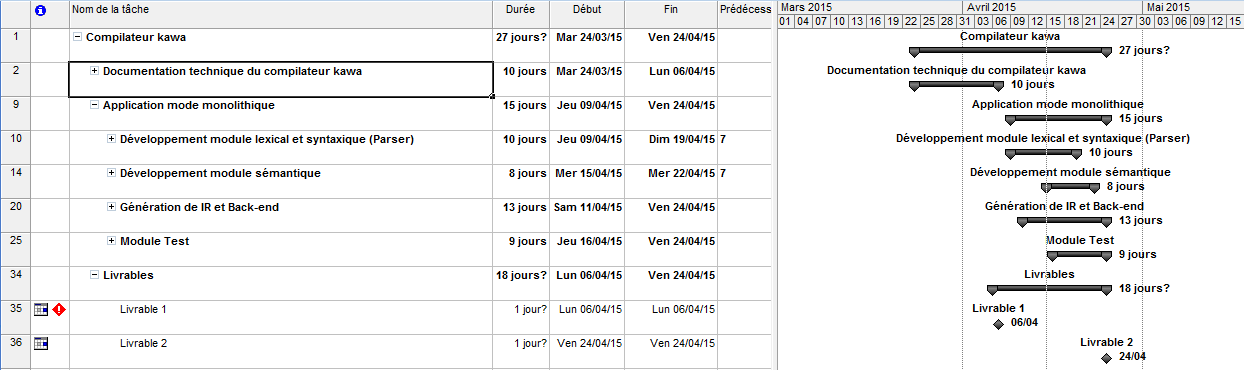
\includegraphics[width=17.8cm]{img_Gantt/Gantt_Global.PNG}
      \caption{Decoupage général en cycles.}
      \label{decoupage_cycles}
    \end{figure}
    
    \subsection{Découpage du livrable 1}

      \begin{figure}[!h]
        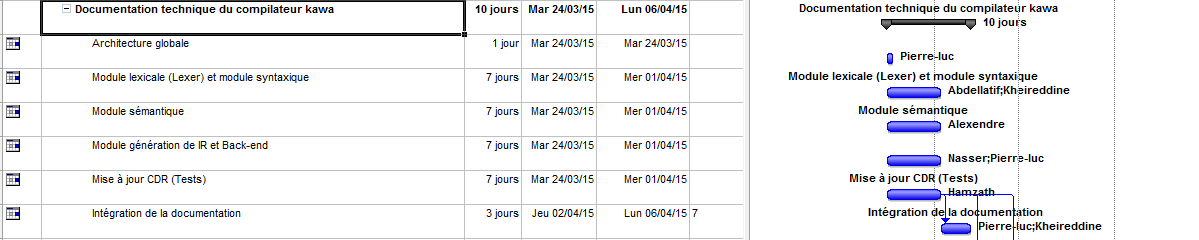
\includegraphics[width=17.8cm]{img_Gantt/Gantt_Livrable1.PNG}
        \caption{Décomposition du cycle pour le livrable 1}
        \label{decomposition_cycle_livrable_1}
      \end{figure}

    \subsection{Découpage du livrable 2}
      \begin{figure}[!h]
        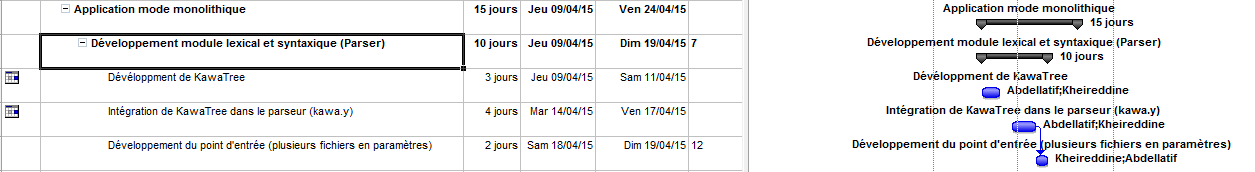
\includegraphics[width=17.8cm]{img_Gantt/Gantt_livrable2_Module_Syntaxe.PNG}
        \caption{Décomposition du cycle pour le module syntaxique}
        \label{decomposition_cycle_livrable_2}
      \end{figure}
      \begin{figure}[!h]
        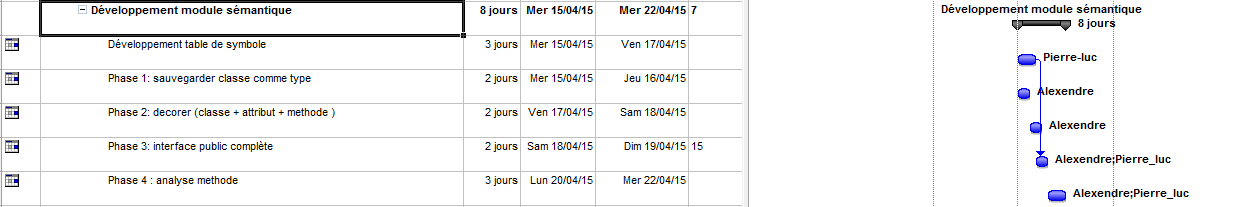
\includegraphics[width=17.8cm]{img_Gantt/Livrable2_Module_Semantique.PNG}
        \caption{Décomposition du cycle pour le module sémantique}
        \label{decomposition_cycle_livrable_2}
      \end{figure}
      \begin{figure}[!h]
        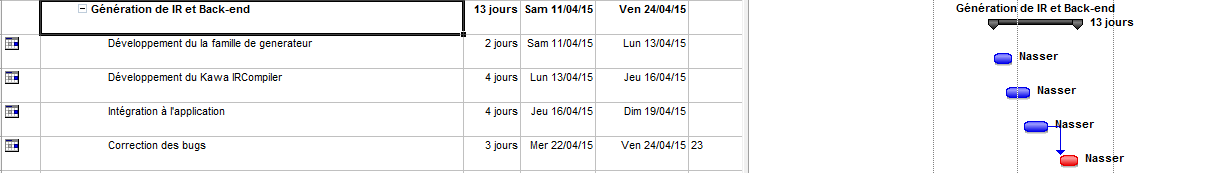
\includegraphics[width=17.8cm]{img_Gantt/Livrable2_Module_BackEnd.PNG}
        \caption{Décomposition du cycle pour le module backend}
        \label{decomposition_cycle_livrable_2}
      \end{figure}
      \begin{figure}[!h]
        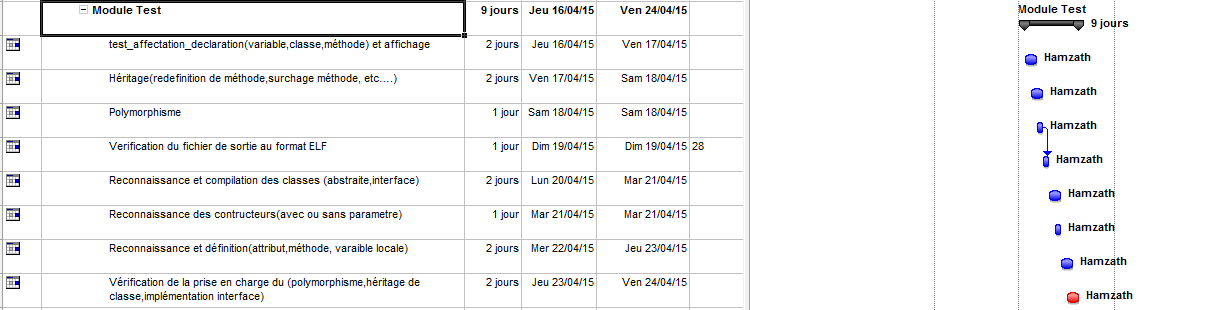
\includegraphics[width=17.8cm]{img_Gantt/Livrable2_Module_Test.PNG}
        \caption{Décomposition du cycle pour le module test}
        \label{decomposition_cycle_livrable_2}
      \end{figure}


  \subsection{Réunion de début d'itération}    
    Cette réunion se fera systématiquement le premier jour du cycle. Elle permet au groupe de se réunir, de fixer les objectifs du cycle ainsi que rappeler les tâches à effectuer par binôme et les dates limites. Elle permet de répondre aux éventuelles interrogations des membres de l’équipe.

  \subsection{Développement et corrections}
    Cette phase comporte plusieurs étapes. Tout d’abord il y a une première phase de développement. Pendant cette phase de développement, des réunions ou contacts réguliers avec le client sont organisés. Il est régulièrement tenu au courant (bilan hebdomadaire) de l’avancement, que ce soit par mail (avec des imprimés écrans montrant les fonctionnalités, ou un site hébergé de manière temporaire et privé), ou par réunion. Le client peut alors tester les fonctionnalités et nous faire parvenir ses retours et impressions. En parallèle, les tests sont effectués à chaque fois qu’une fonctionnalité est développée. Lors d’un retour, (qu’il parvienne du client ou du binôme ayant effectué les tests), les anomalies sont corrigées.
  \subsection{Livraison du produit intermédiaire}
    Cette phase a lieu quelques jours avant la fin de l’itération. C’est lors de cette réunion avec le client que les différents livrables (application et documents) lui sont présentés. Il peut alors nous faire parvenir ses réactions à chaud, ainsi que par mail quelques jours ensuite. De plus, le responsable client transmettra régulièrement par mail l’état de l’avancement du projet aux clients. Enfin, les clients pourront évaluer en temps réel l’avancement de l’application grâce à l’hébergement provisoire et privé mis en place. Ils pourront alors nous faire part de leurs impressions, et remplir le journal de tests s’ils rencontrent des problèmes. Un point client sera alors mis en place régulièrement.
  \subsection{Corrections}
    Après les retours du client, cette phase consiste à apporter les modifications demandées, ainsi que corriger les éventuels bugs détectés.
  \subsection{Réunion de fin d’itération}
    A la fin de chaque cycle aura lieu une réunion de fin d’itération. Elle aura pour but de réaliser un bilan du cycle passé et de déterminer les évolutions à adopter pour les prochains cycles si nécessaires.
  \subsection{Suivi hebdomadaire}
    Durant chaque cycle, une réunion de groupe hebdomadaire aura systématiquement lieu. Durant ces réunions, nous étudierons l’avancement des différentes tâches, nous évoquerons les éventuelles difficultés rencontrées et tenterons d’y trouver une solution. Des réunions supplémentaires pourront être fixées si nécessaire.
  \subsection{Versionning}
    À la fin de chacun de ces cycles sera livrée une version intermédiaire du logiciel. Nous livrerons donc trois versions du logiciel au client.
    \begin{itemize}
      \item 19/04/15 : Version 0.5
      \item 24/04/15 : Version 1.0
    \end{itemize}
  \subsection{Documents}
    Les différents documents doivent être tenus à jour tout au long du projet. Pour chaque action effectuée, chaque membre du projet est tenu de compléter les documents correspondants.
  \newpage
%% ------ Fin section ---------------------------------------------------------
\section{Organisation et responsabilité}
Notre équipe de projet est composée de sept personnes suivant l’organigramme suivant :
 \begin{figure}[!h]
    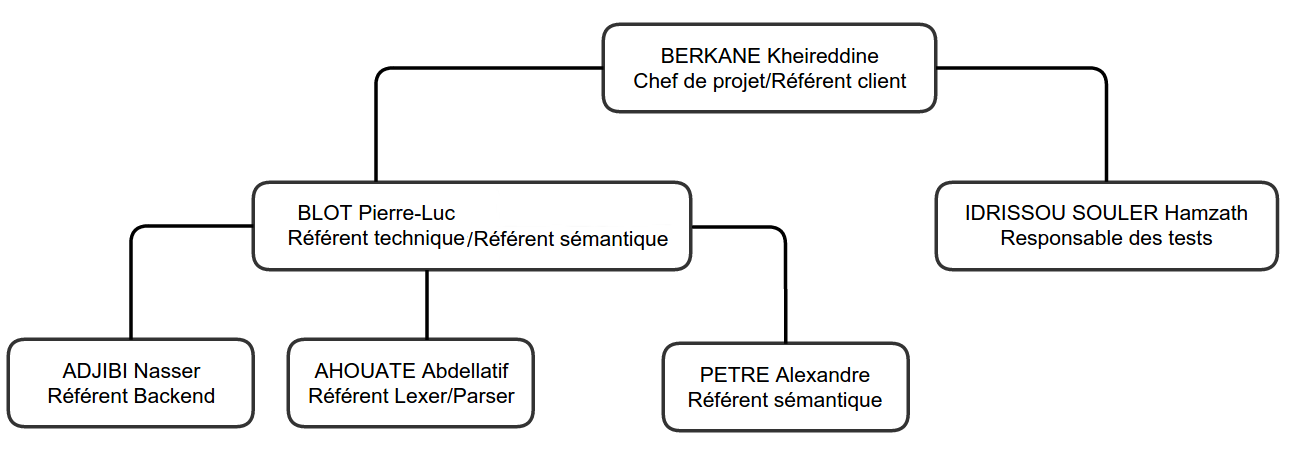
\includegraphics[width=17.8cm]{fig/organigramme-v2.png}
    \caption{Organigramme}
    \label{organigramme}
  \end{figure}

  \subsection{Attribution des rôles au sein de l’équipe de développement}
    Nous avons décidé de répartir les rôles de manière équitable. En effet, chaque membre du groupe est un développeur mais possède également un rôle plus précis qui implique des responsabilités.
  \subsection{Chef de projet}
    Le chef de projet est le support de l’équipe. En effet il est le coordinateur de l’équipe car il doit mener le projet et gérer son bon déroulement. Pour cela, il doit estimer et planifier les phases de développement ainsi qu’assurer la qualité du logiciel. Le chef de projet est amené à suivre l’avancement du projet. De plus, il anime l’équipe et s’occupe de la communication entre les membres de l’équipe et doit gérer les éventuels problèmes. Pierre-Luc a été désigné chef de projet, pour ses capacités d’encadrement, son organisation et sa rigueur. Et a tenu ce rôle jusqu'au 18/02/2015. Pour des raisons personnelles il n'a plus été en mesure d'assurer la gestion de l'équipe. C'est pourquoi Kheireddine BERKANE qui était suppléant pour ce rôle a été désigné chef de projet.
  \subsection{Chargé client}
    Le chargé client représente l’équipe auprès du client. Il a une vision à la fois technique et générale du projet. Il est amené à communiquer avec le client pour lister ses besoins et définir les ordres du jour lors des réunions. Il doit informer le client sur l’avancement du projet et maintenir le contact avec lui tout au long du projet.
    Kheireddine a été désigné chargé client car il aime le contact et communique aisément. Pierre-Luc a été désigné chargé client suppléant en cas d’absence de Kheireddine.
  \subsection{Testeur}
    Le testeur s’occupe de la planification, la création et la réalisation des tests. Il est chargé de produire des rapports réguliers décrivant les erreurs trouvées dans le produit. Dans ce rapport doivent figurer les étapes nécessaires pour reproduire le bug. De ce fait, il doit faire remonter tous les problèmes rencontrés lors des tests le plus rapidement possible au chef de projet. Son principal rôle est donc de vérifier le bon fonctionnement du logiciel. Alexandre a été désigné testeur pour ses connaissances en POO. Pour les même raisons, Hamzath et Abdallatif ont également été désignés. Suite au départ d'un membre de l'équipe et de nouvelles tâches a réaliser, le rôle de testeur a été attribué à Hamzath.
  \subsection{Responsable technique et développement}
    Le responsable technique et développement est l’expert technique du projet. Il est chargé de modéliser les différents composants et créer le modèle d’architecture logicielle. Il doit pour cela comprendre le fonctionnement interne de l’application. C’est lui qui est également chargé de définir les éventuelels API qui vont être utilisés ainsi que les différents langages de programmation. Il doit être une référence pour les autres développeurs dans les langages et API qu’il a choisi. Nasser a été désigné responsable technique et développement car il a de bonnes connaissances LLVM et il les maintient à jour régulièrement. De plus, il a un esprit synthétique permettant de définir clairement les différents composants. Pour les mêmes raisons, Majid a également été désignée sur ce rôle.\\
    Les membres qui sont rataché a ce rôle ont beaucoup changé puisque Majid ne faisant plus partie de l'équipe et le besoin de recherches plus approfondies ont conduit à l'organisation suivante. Nasser est responsable de la partie concernant le Backend du compilateur. Kheireddine et Abdellatif sont responsable de la partie Frontend du compilateur, l'analyseur syntaxique (lexer et parser). Et enfin Alexandre et Pierre-Luc sont responsable de l'analyseur sémantique du compilateur. De plus, Pierre-Luc a le rôle de superviser et la partie Backend.
  \subsection{Développeur, programmeur}
    Le développeur, programmeur doit suivre les différentes directives du responsable technique et du chef de projet. Il est amené à proposer des idées d’amélioration. Il est chargé de développer l’application en respectant les différents documents livrables. Il doit corriger les erreurs remontées lors des différents tests. Il doit avoir des connaissances dans les langages et API utilisés, ou se former si nécessaire. Nous sommes tous développeur, programmeur en plus de nos précédents rôles. 
  %\subsection{Manager}
  % Le manager joue un rôle de conseiller extérieur. Il fournit un ensemble de méthodes et nous guide tout au long du projet. Ceci dans le but d'aider l'équipe à acquérir les points clés nécessaires au bon déroulement du projet. Il est également présent pour mesurer l'avancement du projet et nous signaler d’éventuels écarts ou manquements à nos devoirs afin de nous aiguiller. Le manager possède une aisance pour la communication et pour l’enseignement. Il dispose de connaissances à la fois générales et techniques. Notre manager est Karim Abdellah Godard. 
  \subsection{Client}
    Le client fait appel à nos services pour nous exposer son besoin. Il nous accompagne au maximum tout au long du projet pour nous faire part de ses remarques et valider notre travail. Il est également présent pour tester les fonctionnalités et remonter d’éventuels problèmes à la fin de chaque cycle de développement. Son étroite collaboration tout au long du projet doit permettre aux développeurs d’aller dans son sens dans le but de zproduire un travail qui réponde le plus possible au besoin initial.
      Notre client est Mr Nicart.
  \subsection{Professeur référent}
    Le professeur référant agit comme une interface entre l'équipe de développement et le client. Il nous aide à comprendre son besoin, à le contacter et à établir des moments de rencontre. Il suit l'avancement de notre travail et le valide. Notre professeur référent est Mr Nicart.

%\section{Organigramme des tâches}
%  Nous obtenons alors l’organigramme des tâches suivant :
  \newpage
%% ------ Fin section ---------------------------------------------------------
\section{Procédés de gestion}
  \subsection{Gestion de la documentation}
    Différent documents sont à produire pendant le projet, en voici la liste et le détail des responsabilités.\\

    \subsubsection{Spécification Technique du besoin (STB)}
    \begin{tabular}{
        |>{\centering}p{7,5cm}
        |>{\centering}p{7,5cm}|}
          \hline
          \color{white}\cellcolor{blue}\bfseries{Nom}&
          \color{white}\cellcolor{blue}\bfseries{Spécification Technique du Besoin (STB)}\\
          \cr
          \hline
          But du document &
            \begin{itemize}
              \item Traduire les besoins des utilisateurs et établir une référence pour sa validation
              \item Recenser les exigences que l'équipe de développement s'engage à satisfaire.
            \end{itemize}
          \cr
          \hline
          Responsabilités de rédaction & 
          \begin{itemize}
            \item ADJIBI Nasser
            \item BERKANE Kheireddine
          \end{itemize}
          \cr
          \hline
          Responsabilité de relecture &
          \begin{itemize}
            \item BLOT Pierre-Luc
            \item PETRE Alexandre
          \end{itemize}
          \cr
          \hline
          Appobation requise & Mr Nicart
          \cr
          \hline
    \end{tabular}\\
    
    \subsubsection{Description Architecture Logicielle}
    \begin{tabular}{
        |>{\centering}p{7,5cm}
        |>{\centering}p{7,5cm}|}
          \hline
          \color{white}\cellcolor{blue}\bfseries{Nom}&
          \color{white}\cellcolor{blue}\bfseries{Description Architecture Logicielle}\\
          \cr
          \hline
          But du document &
            \begin{itemize}
              \item Décrire les solutions techniques pour répondre aux exigences
              \item Description et identification des différents modules ou constituants logiciel ainsi que leurs interfaces.
            \end{itemize}
          \cr
          \hline
          Responsabilités de rédaction & 
          \begin{itemize}
            \item ADJIBI Nasser
            \item PETRE Alexandre
            \item BLOT Pierre-Luc
            \item BERKANE Kheireddine
            \item IDRISSOU Hamzath
            \item AHOUATE Abdellatif
          \end{itemize}
          \cr
          \hline
          Responsabilité de relecture &
          \begin{itemize}
            \item ADJIBI Nasser
            \item PETRE Alexandre
            \item BLOT Pierre-Luc
            \item BERKANE Kheireddine
            \item IDRISSOU Hamzath
            \item AHOUATE Abdellatif
          \end{itemize}
          \cr
          \hline
          Appobation requise & Mr Nicart
          \cr
          \hline
    \end{tabular}\\
    
    \subsubsection{Cahier de recettes}
    \begin{tabular}{
        |>{\centering}p{7,5cm}
        |>{\centering}p{7,5cm}|}
          \hline
          \color{white}\cellcolor{blue}\bfseries{Nom}&
          \color{white}\cellcolor{blue}\bfseries{Cahier de Recettes (CdR)}\\
          \cr
          \hline
          But du document &
            \begin{itemize}
              \item Définition des moyens et procédés mis en oeuvre pour assurer la recette du logiciel développé.
              \item Vérifier que le logiciel est conforme à la spécification technique du besoin.
              \item Recenser les objectifs de tests de validation et les moyens nécessaires pour les atteindre.
            \end{itemize}
          \cr
          \hline
          Responsabilités de rédaction & 
          \begin{itemize}
            \item PETRE Alexandre
            \item IDRISSOU Hamzath
          \end{itemize}
          \cr
          \hline
          Responsabilité de relecture &
          \begin{itemize}
            \item BLOT Pierre-Luc
          \end{itemize}
          \cr
          \hline
          Appobation requise & Mr Nicart
          \cr
          \hline
    \end{tabular}\\

    \subsubsection{Analyse des Risques (AdR)}
    \begin{tabular}{
        |>{\centering}p{7,5cm}
        |>{\centering}p{7,5cm}|}
          \hline
          \color{white}\cellcolor{blue}\bfseries{Nom}&
          \color{white}\cellcolor{blue}\bfseries{Analyse des Risques (AdR)}\\
          \cr
          \hline
          But du document &
            \begin{itemize}
              \item Recenser les risques ainsi que leurs probabilités.
              \item Les actions à effectuer en cas de réalisation de ces risques.
            \end{itemize}
          \cr
          \hline
          Responsabilités de rédaction & 
          \begin{itemize}
           \item BLOT Pierre-Luc
          \end{itemize}
          \cr
          \hline
          Responsabilité de relecture &
          \begin{itemize}
            \item BERKANE Kheireddine
          \end{itemize}
          \cr
          \hline
          Appobation requise & Mr Nicart
          \cr
          \hline
    \end{tabular}\\

    \subsubsection{Plan de Développement (PdD)}
    \begin{tabular}{
        |>{\centering}p{7,5cm}
        |>{\centering}p{7,5cm}|}
          \hline
          \color{white}\cellcolor{blue}\bfseries{Nom}&
          \color{white}\cellcolor{blue}\bfseries{Plan de Développement (PdD)}\\
          \cr
          \hline
          But du document &
            \begin{itemize}
              \item Décrire l'organisation du projet et les règles de gestion.
            \end{itemize}
          \cr
          \hline
          Responsabilités de rédaction & 
          \begin{itemize}
            \item BLOT Pierre-Luc
            \item BERKANE Kheireddine
          \end{itemize}
          \cr
          \hline
          Responsabilité de relecture &
          \begin{itemize}
            \item ADJIBI Nasser
          \end{itemize}
          \cr
          \hline
          Appobation requise &
          \begin{itemize}
            \item Mr Nicart
            \item Mr Abdellah
          \end{itemize}
          \cr
          \hline
    \end{tabular}\\

    \subsubsection{Manuel d'utilisation}
    \begin{tabular}{
        |>{\centering}p{7,5cm}
        |>{\centering}p{7,5cm}|}
          \hline
          \color{white}\cellcolor{blue}\bfseries{Nom}&
          \color{white}\cellcolor{blue}\bfseries{Manuel d'utilisation}\\
          \cr
          \hline
          But du document &
            \begin{itemize}
              \item Expliquer l'utilisation du compilateur.
            \end{itemize}
          \cr
          \hline
          Responsabilités de rédaction & 
          \begin{itemize}
            \item ADJIBI Nasser
            \item PETRE Alexandre
            \item BLOT Pierre-Luc
            \item BERKANE Kheireddine
            \item IDRISSOU Hamzath
            \item AHOUATE Abdellatif
          \end{itemize}
          \cr
          \hline
          Responsabilité de relecture &
          \begin{itemize}
            \item ADJIBI Nasser
            \item PETRE Alexandre
            \item BLOT Pierre-Luc
            \item BERKANE Kheireddine
            \item IDRISSOU Hamzath
            \item AHOUATE Abdellatif
          \end{itemize}
          \cr
          \hline
          Appobation requise & Mr Nicart
          \cr
          \hline
    \end{tabular}\\

  \subsection{Gestion des configurations}
    Les documents sont stockés dans un dépôt git privé sur gitlab. Tous les membres de l'équipe y ont accès. Cela nous permet d'obtenir les documents rapidement et dans leurs versions les plus récentes. Chaque personne doit rédiger au moins un document et un document ne doit pas être rédigé par plus de deux personnes. Les versions des documents doivent être relues par l'ensemble de l'équipe (et donc corrigé si nécessaire) avant d'être soumises au client et aux professeurs concernés.\\

    Les sources sont hébergées également sur gitlab. Cela nous permettra d'avoir une version centralisée dans le dépôt git à laquelle tous les membres du groupe pourront accéder. De plus, nous aurons nos propres versions sur nos ordinateurs sur des copies du dépôt git. Cela limite très fortement les risques de perte de données. De plus git permet de gérer les versions par commit ou par tag.\\
    \indent Les membres de l'équipe seront chargés de mettre en ligne leurs fichiers développés en ayant vérifié sur leur version de l'application que l'intégration ne posait pas de problème. Le tout doit ce faire sur la branche global du dépôt git.\\
    \indent Cette branche global contient l'avancement du projet, elle peut contenir des bugs. Dès qu'une version sans bug est implémentée, alors on fusionne la branche global sur la branche master. Ainsi, la branche master contient seulement les versions du projet qui sont fonctionnelles et correctes.\\
    \indent L'intégration se fera automatiquement puisque grâce à git nous pouvons directement travailler par itération sur plusieurs branches paralèlles pour enfin toutes les fusionner au moment voulu. Ces fusions seront coordonnées par le responsable technique.\\

    De plus, l'équipe travail slack. Slack est une plateforme sur laquelle tous les membres de l'équipe sont inscrit. Slack permet aux membres de l'équipe de communiquer via une messagerie instantannée organisée en chaîne de discussion. Slack permet de conserver les historiques de conversation, d'échanger des fichiers, de connecter le compte gitlab sur une chaîne. Ainsi dès que des modifications sont apportées sur le dépôt git en ligne, une notification apparaît avec les trois derniers commit effectués.\\
    \indent Slack peut être installé sur smartphone, et cela offre une grande flexibilité et offre une meilleure communication.\\

    Le client peut accéder au dépôt privé sur gitlab et reçoit par mail une notification dès qu'une version du projet est pushée sur le dépôt en ligne.

\section{Revues et points clefs}
  Voici un récapitulatif rapide de l’ensemble des dates clés du projet kawa. Cette liste n’est pas exhaustive et les dates peuvent être amenées à changer en cours de projet.\\

  \begin{tabular}{
        |>{\centering}p{7,5cm}
        |>{\centering}p{7,5cm}|}
          \hline
          \color{white}\cellcolor{blue}\bfseries{Dates}&
          \color{white}\cellcolor{blue}\bfseries{Evénements}\\
          \cr
          \hline
          17/10/14 & Remise du sujet
          \cr
          \hline
          06/01/15 & Remise des documents v1.0 : AdR, CdR, DAL, PdD et STB
          \cr
          \hline
          19/01/15 & Revue de lancement du projet
          \cr
          \hline
          20/01/15 & Début de la phase de développement
          \cr
          \hline
          19/04/15 & Premier livrable
          \cr
          \hline
          24/04/15 & Second livrable
          \cr
          \hline
    \end{tabular}\\

\end{document}
